\section{Models}\label{sect:method}
\lhead{\textit{Models}}

As previously alluded to in \cref{fig:hesse}, the models that follow rely on an opinion being formed of a probability mass being assigned to a set of possible worlds. For illustrative purposes, consider the $3$ dimensional case above. The opinion of an agent at time $t$ can then be represented in a vector of the form:

\begin{center}
$P^t = \begin{bmatrix}
    p_{1}\\
    p_{2}\\
    p_{3}
\end{bmatrix}$
\end{center}

where $P_i$ reflects the probability mass placed by the agent in question upon state $s_i$. By the axiom $P(W) = 1$, the vector $P^t$ must also sum to $1$. This allows us to form a right-stochastic matrix\footnote{A right stochastic matrix is defined as a square, non-negative matrix for which the rows sum to $1$~\cite{Gagniuc2017MarkovExperimentation}.}, representing the collective beliefs over $n$ states of the world of the full population of $K$ agents at time $t$:

\begin{center}
$\mathbf{P}^t = \begin{bmatrix}
    P_{11} & P_{12} & P_{13} & \dots  & P_{1n} \\
    P_{21} & P_{22} & P_{23} & \dots  & P_{2n} \\
    \vdots & \vdots & \vdots & \ddots & \vdots \\
    P_{K1} & P_{K2} & P_{K3} & \dots  & P_{Kn}
\end{bmatrix}$
\end{center}

Each of the $K$ agents is initialised with $n$ distinct beliefs computed by drawing $n-1$ numbers on the interval $ [ 0,1 ] $. These numbers are sorted and the interval between them yields the initial set of beliefs $P_{k}^0$. In the $3$-dimensional case, at any given time, the beliefs of an agent can be represented as a point on the blue surface in \cref{fig:3d-simplex}. This can be projected down to a $2$-dimensional plot such as those shown as shown in~\cref{fig:2d-simplex}.  In this plot, an agent in the corner of the triangle could be described as being certain, extremist, or having a strong belief in a single hypothesis. Alternatively, those more toward the centre have a relatively uniform distribution in probability space and so would be uncertain or have a weak belief.  

\todo{Correct the vertex labels on this plot}
\begin{figure}
\begin{minipage}[ht]{0.45\textwidth}
    \centering
    \resizebox{\linewidth}{0.74\linewidth}{
   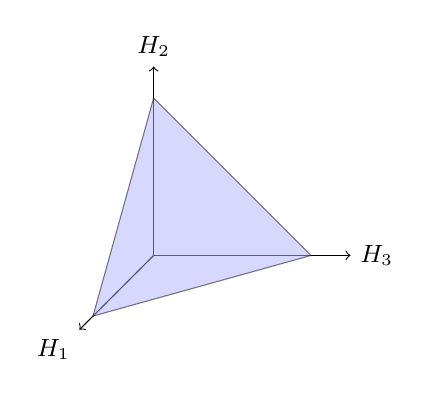
\begin{tikzpicture}[line join = round, line cap = round]
\coordinate [] (A) at (2,0,0);
\coordinate [] (B) at (0,0,2);
\coordinate [] (C) at (0,2,0);
\coordinate [] (D) at (0,0,0);

\draw[->] (0,0) -- (2.5,0,0) node[right] {\small $H_3$};
\draw[->] (0,0) -- (0,2.4,0) node[above] {\small $H_2$};
\draw[->] (0,0) -- (0,0,2.45) node[below left] {\small $H_1$};
\foreach \i in {A,B,C,D}
    \draw[dashed] (0,0)--(\i);
\draw[-, fill=blue!30, opacity=.5] (A)--(B)--(C)--cycle;
\end{tikzpicture} }
\subcaption{$3$-dimensional simplex}\label{fig:3d-simplex}
\end{minipage}
\hfill
  \begin{minipage}[ht]{0.45\textwidth}
    \includegraphics[width=\textwidth]{Images/Figures/OpenModel/open_model_BC_n_3_p_100_gullibility_0,3_runs_10.png} 
    \subcaption{$2$-dimensional projection}\label{fig:2d-simplex}
 \end{minipage}
\caption{An example of a $3$-dimensional simplex over a world with $3$ possible states, projected down to $2$-dimensions. } 
\end{figure}

Once the population is initialised, the lanes of communication must be described. Parker and Zhang describe a characteristic of their model they name the ``well-stirred'' assumption. This assumes that the population is sufficiently mixed together that it is acceptable to select agents at random. This can be thought of in a similar way to the social lattice described in~\cite{Deffuant2000MixingAgents}, though instead of a simple square lattice, the network is fully connected with communicating pairs selected at random. Two agents are drawn randomly from the population, one to be the speaker, one to be the listener. This model is based on a special case of the convention set out by~\cite{Lewis2002ConventionStudy}. This work describes a communicator that acts in its best interests to convey a message that reflects a state of the world that it perceives to be true. This communicator broadcasts its message to an audience that in our case is only one agent but could be generalised to many and, subsequently, the audience performs an action based on the communication it receives. In our case, this is represented in \cref{fig:simple_interaction}. The communication created by the speaker is an argument it hopes will persuade the listener to take some action that will update its beliefs to more closely align to the speaker's. 

 \begin{figure}[H]
 	\centering
 	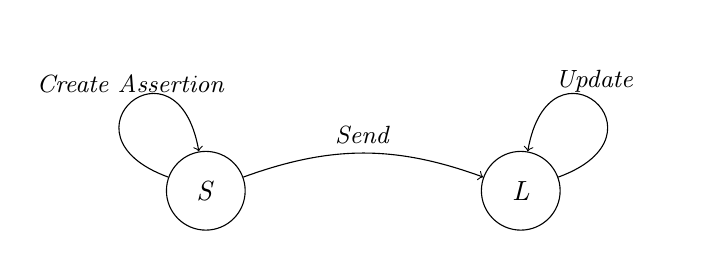
\begin{tikzpicture}[baseline=(S.base)]
 		\tikzset{every loop/.style={min distance=10mm,looseness=10}}
 		\node (S) at (0, 0) [shape=circle,draw,minimum size=1cm] {\textit{S}};
 		\node (L) at (4, 0) [shape=circle,draw, minimum size=1cm] {\textit{L}};
 		\path[->] (S) edge[bend left = 20] node[above]{\small \textit{Send}} (L)
 		edge[loop above,in=100,out=160, min distance=8mm,looseness=8] node{\small \textit{Create Assertion}} (S)
 		(L) edge[loop above,in=80,out=20, min distance=8mm,looseness=8] node{\small \textit{Update}} (L);
 	\end{tikzpicture}
 	\caption{Simple model of the interaction between two agents. \textit{S} is the speaker and \textit{L} is the listener. \textit{S} creates an argument that it then sends to \textit{L}. \textit{L} may then update its own beliefs according to the argument it receives from \textit{S}.}
 	\label{fig:simple_interaction}
 \end{figure}
 
Initially, it is assumed that the speaker will be aware of the listener's opinions prior to communicating the argument and how the listener will react upon hearing it. This process is repeated iteratively until either we reach the maximum number of iterations or the system can be said to have converged, as defined in~\cref{eq:shannon_entropy}. It is the aim of the speaker to share its opinion on the states of the world it believes to be true with the listener in the hopes that the listener will change its attitude to more closely resemble that of the speaker. 



\begin{algorithm}[H]
\SetAlgoLined
\KwResult{Simulation of agent based communication }
 initialization\;
 \While{$i < t_{max}$}{
  selectSpeaker\;
  selectListener\;
  speakerConstructArgument\;
  listenerReactToArgument\;
  \eIf{Converged}{
   break\;
   }{
   i++\;
  }
 }
 \caption{Method}
\end{algorithm}

There are several features that can be useful in determining the dynamics of this system. The average entropy of the population as a whole denotes the level to which the agents have become certain in a single state~\cite{Shannon1948ACommunication}. This is defined as

\begin{equation}\label{eq:shannon_entropy}
    \hat{E}^t = \frac{1}{K} \sum_i^K - \mathbf{P}^t_i \cdot \log ( \mathbf{P}^t_i)
\end{equation}

The system is said to have converged when the entropy has not changed by more than $\eta $ for $T$ iterations, expressed as $\Delta \hat{E}^T = \abs{ \hat{E}^t -  \hat{E}^{t+T}}  \leq \eta$. However, entropy only highlights whether or not the agents hold strong beliefs, not that they agree on those beliefs. Hence, the J-Divergence is used as a symmetric version of KL-Divergence, used to determine the average distance between all pairs of agents in probability space~\cite{Johnson2001SymmetrizingDistance}. It is defined as

\begin{equation}
    \hat{J}_{t} = \frac{1}{K} \sum_j^K \frac{1}{K} \sum_i^K  \frac{1}{2} \left( \mathbf{P}^t_i \log \left( \frac{ \frac{1}{2} (\mathbf{P}^t_i + \mathbf{P}^t_j) }{\mathbf{P}^t_i} \right) +  \mathbf{P}^t_j \log \left( \frac{ \frac{1}{2} (\mathbf{P}^t_i + \mathbf{P}^t_j) }{\mathbf{P}^t_j} \right) \right)
\end{equation}

There are two parts of this model that we will explore. Firstly, we shall consider methods by which a speaker can construct an assertion, increasing in their complexity from openly revealing an agents underlying probability distribution to tailoring the speakers assertion to the listener. Secondly, we define four actions the listener can take, empowering them to react to arguments in a variety of ways, either passively, with discernment or with steadily less and less importance placed on new information as time passes.







